\chapter{Neural Networks}

Neural networks are a set of algorithms, modeled loosely after the human brain, that are designed to recognize patterns. They interpret sensory data through a kind of machine perception, labeling or clustering raw input. The patterns they recognize are numerical, contained in vectors, into which all real-world data, be it images, sound, text or time series, must be translated.\\

Neural networks help us cluster and classify. You can think of them as a clustering and classification layer on top of the data you store and manage. They help to group unlabeled data according to similarities among the example inputs, and they classify data when they have a labeled dataset to train on. \\

\section{Model Representation}

Let's examine how we will represent a hypothesis function using neural networks. At a very simple level, neurons are basically computational units that take inputs (dendrites) as electrical inputs (called "spikes") that are channeled to outputs (axons). In our model, our dendrites are like the input features $x_1\dots x_n$, and the output is the result of our hypothesis function. In this model our $ x_0 $ input node is sometimes called the "bias unit." It is always equal to 1. In neural networks, we use the same logistic function as in classification, $ \frac{1}{1 + e^{-\theta^Tx}} $, yet we sometimes call it a sigmoid (logistic) activation function. In this situation, our "theta" parameters are sometimes called "weights".\\

\begin{figure}[h!]
	\centering
	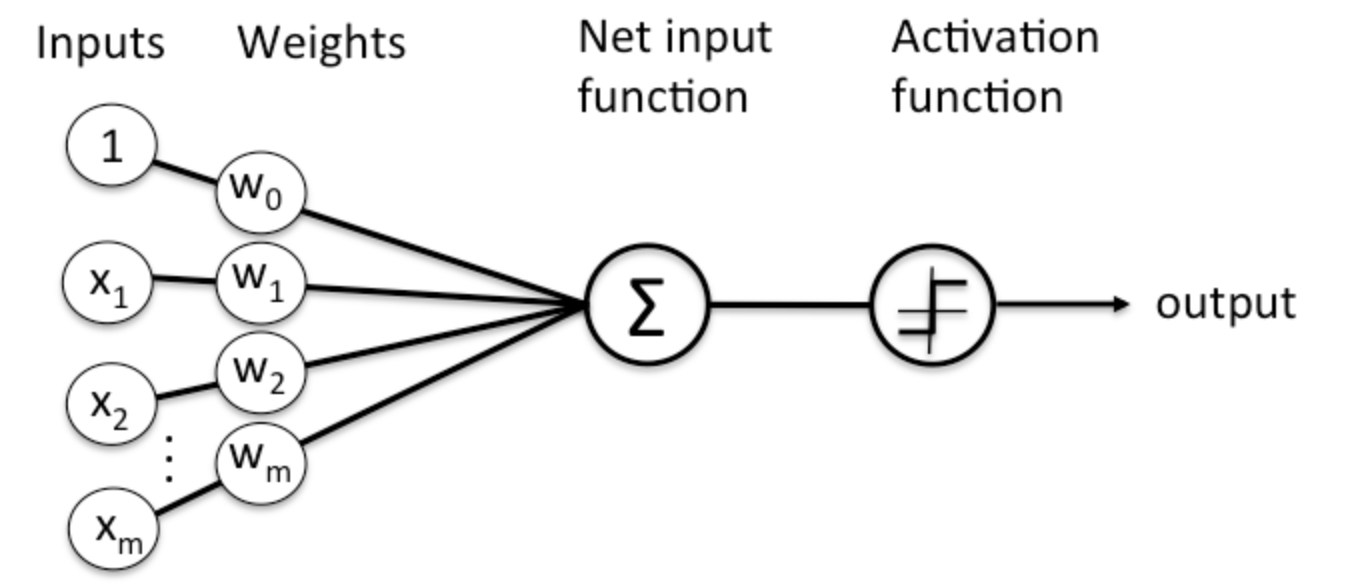
\includegraphics[width=0.7\textwidth]{fig/neural_diag}
	\caption{Neural diagram}
\end{figure}

\pagebreak

Visually, a simplistic representation looks like:\\

\begin{align*}
\begin{bmatrix}
x_{1} \\
x_{2} \\
\vdots \\
x_{n}
\end{bmatrix}
\rightarrow
[ \hspace{0.5cm}]
\rightarrow  h_\theta (x)
\end{align*}

Our input nodes (layer 1), also known as the "input layer", go into another node (layer 2), which finally outputs the hypothesis function, known as the "output layer".We can have intermediate layers of nodes between the input and output layers called the "hidden layers."

\begin{figure}[h!]
	\centering
	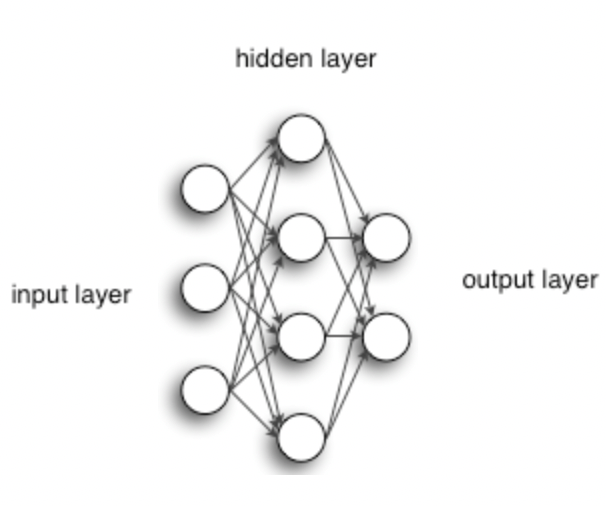
\includegraphics[width=0.5\textwidth]{fig/neural_net}
	\caption{Neural layers}
\end{figure}

Where:

\begin{itemize}
\item $ a^{(j)}_i $ = "\textbf{activation}" of unit \textit{i} in layer \textit{j}\\
\item $\Theta ^{(j)} $=matrix of \textbf{weights} controlling function mapping from layer \textit{j} to layer \textit{j+1}
\end{itemize}

If we had one hidden layer, with \textbf{3} activations,  it would look like:

\begin{align*}
\begin{bmatrix}
x_{0}\\
x_{1} \\
x_{2} \\
x_{3}
\end{bmatrix}
\rightarrow
\begin{bmatrix}
\vspace{0.15cm}a_{1}^{(2)}\\\vspace{0.15cm}
a_{2}^{(2)} \\
a_{3}^{(2)}
\end{bmatrix}
\rightarrow  h_\theta (x)
\end{align*}

The values for each of the "activation" nodes is obtained as follows:

\begin{align*}
a^{(2)}_1&=g\left(\Theta^{(1)}_{10}x_0+\Theta^{(1)}_{11}x_1+\Theta^{(1)}_{12}x_2+\Theta^{(1)}_{13}x_3\right)\\
a^{(2)}_2&=g\left(\Theta^{(1)}_{20}x_0+\Theta^{(1)}_{21}x_1+\Theta^{(1)}_{22}x_2+\Theta^{(1)}_{23}x_3\right)\\
a^{(2)}_3&=g\left(\Theta^{(1)}_{30}x_0+\Theta^{(1)}_{31}x_1+\Theta^{(1)}_{32}x_2+\Theta^{(1)}_{33}x_3\right)\\
h\Theta^(x_)=a^{(3)} _1&=g\left(\Theta^{(2)}_{10}a^{(2)}_0+\Theta^{(2)}_{11}a^{(2)}_1+\Theta^{(2)}_{12}a^{(2)}_2+\Theta^{(2)}_{13}a^{(2)}_3\right)
\end{align*}

This is saying that we compute our activation nodes by using a \textit{3x4} matrix of parameters. We apply each row of the parameters to our inputs to obtain the value for one activation node. Our hypothesis output is the logistic function applied to the sum of the values of our activation nodes, which have been multiplied by yet another parameter matrix $ \Theta ˆ{(2)} $ containing the weights for our second layer of nodes. And each layer gets its own matrix of weights, $ \Theta ^{(j)} $.\\

The dimensions of these matrices of weights is determined as follows:\\

\begin{tcolorbox}[width=\textwidth,colback={white},colbacktitle=white]
If network has $ s_j $ units in layer $ j $ and $ s_{j+1} $  units in layer $ j+1 $, then $ \Theta^{(j)} $ will be of dimension $ s_{j+1} \times (s_j+1) $.
\end{tcolorbox}

\vspace{0.5cm}

The \textbf{+1} comes from the addition in $ \Theta ^{(j)} $ of the "\textbf{bias nodes}", $ x_0 $ and $ \Theta ^{(j)}_0 $. In other words the output nodes will not include the bias nodes while the inputs will.

\subsection{Vectorized implementation}

We're going to define a new variable $ z_k^{(j)} $ that encompasses the parameters inside our \textbf{g} function. In our previous example if we replaced by the variable \textbf{z} for all the parameters we would get:

\begin{align*}
a^{(2)}_1&=g\left(z^{(2)}_1  \right)\\
a^{(2)}_2&=g\left(z^{(2)}_2  \right)\\
a^{(2)}_3&=g\left(z^{(2)}_3  \right)
\end{align*}

In other words, for layer $ j=2 $ and node \textbf{k}, the variable \textbf{z} will be:

\begin{center}
$z^{(2)}_k=g\left(\Theta^{(1)}_{k,0}x_0+\Theta^{(1)}_{k,1}x_1+ \dots +\Theta^{(1)}_{k,n}x_n\right)$
\end{center}

Setting the input $ x = a^{(1)} $, we can rewrite the equation as:

\begin{equation}
z^{(j)} = \Theta^{(j-1)}  a^{(j-1)}  
\end{equation}

Now we can get a vector of our activation nodes for layer j as follows:

\begin{equation}
a^{(j)}  = g(z^{(j)})
\end{equation}